\setcounter{section}{4}
\section{Tests for Positive Series}
\begin{Definition}{Positive}{}
    A series $ \sum\limits_{n=1}^{\infty} a_n $ is called \textbf{positive}
    if $ a_n\geqslant 0 $ for all $ n $.
\end{Definition}
There are a few tests that only work on positive series:
\begin{enumerate}[label=(\Roman*)]
    \item Integral Test
    \item Comparison Test
    \item Limit Comparison Test
\end{enumerate}
Let's examine these now!
\subsection*{The Integral Test}
\begin{Theorem}{Integral Test}{int_test}
    Suppose $ f(x) $ is continuous, positive, and decreasing
    for $ x\in\interval[open right]{1}{\infty} $. Let $ a_n=f(n) $. Then,
    $ \sum\limits_{n=1}^{\infty}  $ converges if and only if $ \int_{1}^{\infty} f(x)\odif{x} $
    converges.
\end{Theorem}
\begin{Remark}{}{}
    These three conditions don't need to hold for all $ x\geqslant 1 $, just
    \textbf{eventually} (for $ x\geqslant m $ for some $ m\in\mathbb{R}^+ $),
    which is the case most of the time when dealing with series and improper integrals!
\end{Remark}
\begin{Proof}{\ref{thm:int_test}}{}
    We can cleverly look at two different approximations for the area
    under $ f(x) $ (which is continuous, positive, and decreasing).  $ y=f(x) $,
    $ f(n)=a_n $:
    \begin{center}
        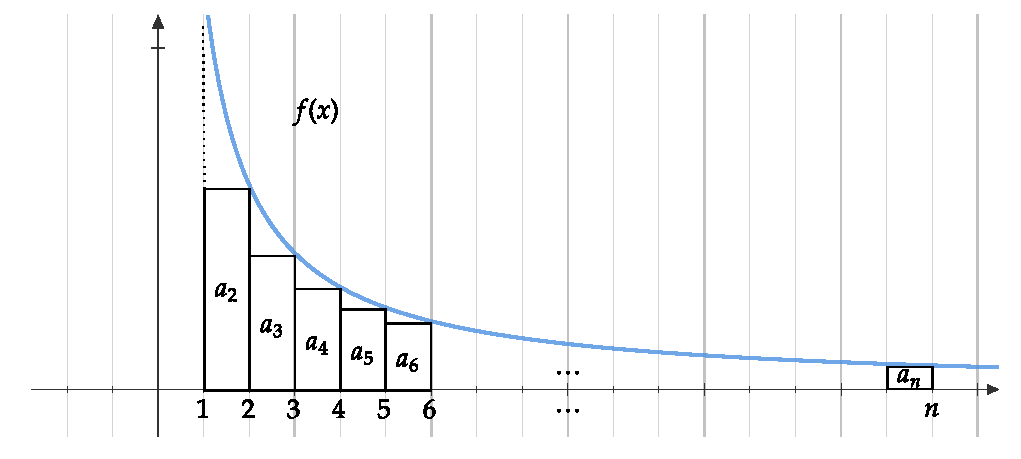
\includegraphics[width=0.49\textwidth]{reimann1.pdf}
        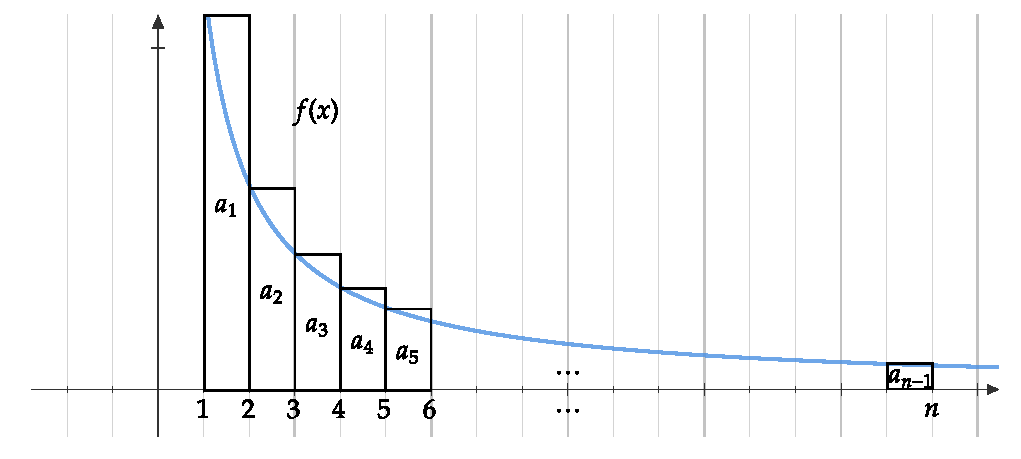
\includegraphics[width=0.49\textwidth]{reimann2.pdf}
    \end{center}
    $ (\star) $ First figure:
    \[ a_2+a_3+a_4+\cdots+a_n\leqslant \int_{1}^{n} f(x)\odif{x} \]
    $ (\star\star) $ Second figure:
    \[ a_1+a_2+\cdots+a_{n-1}\geqslant \int_{1}^{n} f(x)\odif{x} \]
    $ (\impliedby) $ Suppose $ \int_{1}^{\infty} f(x)\odif{x} $ converges. $ (\star) $
    says
    \[ \sum\limits_{k=2}^{n} a_k\leqslant \int_{1}^{n} f(x)\odif{x}\leqslant
        \int_{1}^{\infty} f(x)\odif{x}  \]
    since $ f(x)\geqslant 0 $. So,
    \[ S_n=a_1+\sum\limits_{k=2}^{\infty} a_k\leqslant a_1+\int_{1}^{\infty} f(x)\odif{x}  \]
    which is a constant, say $ M $. So, $ 0\leqslant S_n\leqslant M $ for all $ n $.
    Also, $ S_{n+1}=S_{n}+a_{n+1}\geqslant S_n $ since $ a_{n+1}>0 $. So
    $ \set{S_n} $ is a bounded monotonic sequence! Therefore,
    $ \set{S_n} $ converges by MCT, which means $ \sum\limits_{n=1}^{\infty} a_n $
    converges.

    $ (\implies) $ If $ \int_{1}^{\infty} f(x)\odif{x}  $ diverges, then
    \[ \lim\limits_{{n} \to {\infty}} \int_{1}^{n} f(x)\odif{x} =\infty \]
    and $ (\star\star) $ says
    \[ \int_{1}^{n} f(x)\odif{x}\leqslant \sum\limits_{k=1}^{n-1} a_k=S_{n-1} \]
    so $ \lim\limits_{{n} \to {\infty}} S_{n-1}=\infty $, which means
    $ \sum\limits_{n=1}^{\infty} a_n $ diverges.
\end{Proof}

\begin{Remark}{}{}
    When to use the Integral Test!
    \begin{itemize}
        \item When the series ``looks like'' it can be integrated; that is, when there
              are terms like $ \ln(n) $, $ e^n $, etc.
        \item Compared to other tests, the Integral Test takes longer to use, it is better used
              as a last resort!
    \end{itemize}
\end{Remark}

\begin{Remark}{}{}
    Don't forget to show the function is \emph{continuous}, \emph{positive}, and
    \emph{decreasing}!
\end{Remark}

\begin{Example}{}{}
    Determine whether the following series is convergent or divergent.
    \begin{enumerate}[label=(\roman*)]
        \item $ \displaystyle \sum\limits_{n=1}^{\infty} \frac{1}{n^2} $

              \textbf{Solution.} First, $ \displaystyle  f(x)=\frac{1}{x^2} $ is continuous, positive,
              and decreasing for $ x\geqslant 1 $. So we can apply the Integral Test.
              $ \displaystyle \int_{1}^{\infty} \frac{1}{x^2} \odif{x} $ converges ($ p $-integral
              with $ p=2>1 $), so the series converges.
        \item $  \displaystyle\sum\limits_{n=1}^{\infty} \frac{\ln(n)}{n} $

              \textbf{Solution.} Does the Divergence Test work?
              \[ \lim\limits_{{n} \to {\infty}} \frac{\ln(n)}{n}=
                  \lim\limits_{{n} \to {\infty}} \frac{\sfrac{1}{n}}{1} =0\ldots\text{ no info} \]
              Let $ f(x)=\dfrac{\ln(x)}{x} $, $ f $ is clearly continuous and positive for $ x>1 $,
              but is it decreasing? Let's check!
              \[ f^\prime(x)=\frac{1-\ln(x)}{x^2}=0 \]
              Before $ x=e $, $ f^\prime $ is positive and increasing.

              After $ x=e $, $ f^\prime $ is negative
              and $ f $ is decreasing.

              So, it is decreasing eventually (for $ x\geqslant e $). So,
              we can use the Integral Test!
              \[ \int_{1}^{\infty} \frac{\ln(x)}{x} \odif{x}
                  =\lim\limits_{{b} \to {\infty}} \left[ \frac{\left( \ln(x) \right)^2}{2} \right]_1^b
                  =\lim\limits_{{b} \to {\infty}} \frac{\left( \ln(b) \right)^2}{2}=\infty   \]
              So, the series diverges.
    \end{enumerate}
\end{Example}

Q\@: For which $ p\in\mathbb{R} $ is $ \displaystyle \sum\limits_{n=1}^{\infty} \frac{1}{n^p} $
convergent?

A\@:
\begin{Proof}{\ref{thm:p_test}}{}
    \underline{Case 1}: $ p<0 $. $ \displaystyle \lim\limits_{{n} \to {\infty}} \frac{1}{n^p} =\infty $,
    therefore the series diverges by the Divergence Test.

    \underline{Case 2}: $ p=0 $. $ \displaystyle \lim\limits_{{n} \to {\infty}} \frac{1}{n^0} =1 $,
    therefore the series diverges by the Divergence Test.

    \underline{Case 3}: $ p>0 $. $ f(x)=\dfrac{1}{x^p} $ is continuous, positive, and decreasing
    for $ x\geqslant 1 $. Also, we know $ \displaystyle \int_{1}^{\infty} \frac{1}{x^p} \odif{x} $
    converges if and only if $ p>1 $.
\end{Proof}

\begin{Theorem}{$ p $-Series Test}{p_test}
    The series $ \displaystyle \sum\limits_{n=1}^{\infty} \frac{1}{n^p}  $ converges
    if and only if $ p>1 $, and diverges if $ p\leqslant 1 $.
\end{Theorem}

\begin{Example}{$ p $-Series}{}
    Determine whether the following series is convergent or divergent.
    \begin{itemize}
        \item $ \displaystyle \sum\limits_{n=1}^{\infty} \frac{1}{n^{\sfrac{3}{2} }} $

              \textbf{Solution.} $ p $-series with $ p=\sfrac{3}{2} >1 $,
              therefore the series converges.
        \item $ \displaystyle \sum\limits_{n=1}^{\infty} \frac{1}{\sqrt{n}} $

              \textbf{Solution.} $ p $-series with $ p=\sfrac{1}{2} <1 $, therefore the series
              diverges.
    \end{itemize}
\end{Example}

\begin{Remark}{}{}
    Note that the series does \emph{not} converge to what the integral converges to! For example,
    \[ \sum\limits_{n=1}^{\infty} \frac{1}{n^2} =\frac{\pi^2}{6} \]
    but $ \displaystyle \int_{1}^{\infty} \frac{1}{x^2} \odif{x}=1$.
    However, we \emph{can} use the integral
    test to approximate the sum of a series!
\end{Remark}

\begin{Definition}{Remainder}{}
    The \textbf{remainder} is the error in using $ S_n $ to approximate $ \sum\limits_{n=1}^{\infty} a_n=S $,
    so
    \[ R_n=S-S_n=a_{n+1}+a_{n+2}+\cdots \]
    If $ a_n=f(n) $ and $ f(x) $ is continuous, positive, and decreasing, we know that
    \[ \boxed{\int_{n+1}^{\infty} f(x)\odif{x} \leqslant R_n\leqslant \int_{n}^{\infty} f(x)\odif{x}} \]
    from the proof of the Integral Test.
\end{Definition}
So we get an upper bound on the remainder!

\begin{Example}{}{}
    Find an upper bound on the error if we use $ S_{10} $ to approximate
    $ \displaystyle\sum\limits_{n=1}^{\infty} \frac{1}{n^2}  $.

    \textbf{Solution.} $ \displaystyle R_{10}\leqslant \int_{10}^{\infty}\frac{1}{x^2}  \odif{x}=
        \text{exercise}=\sfrac{1}{10} $, so the error is at most $ 0.1 $.
\end{Example}

\begin{Example}{}{}
    How many terms are needed to approximate $ \displaystyle \sum\limits_{n=1}^{\infty} \frac{1}{n^2}  $
    with an error of at most $ 0.001 $?

    \textbf{Solution.} Need $ R_n\leqslant 0.001 $, but we know $
        \displaystyle R_n\leqslant \int_{n}^{\infty}
        \frac{1}{x^2} \odif{x} $, so solve
    \[ \int_{n}^{\infty} \frac{1}{x^2} \odif{x} \leqslant 0.001\implies
        \frac{1}{n} \leqslant 0.001\implies n\geqslant 1000 \]
\end{Example}

We can improve our estimate, rather than just using $ S_n $:
\[ \int_{n+1}^{\infty} f(x)\odif{x} \leqslant R_n=S-S_n\leqslant \int_{n}^{\infty} f(x)\odif{x} \]
so
\[ S_n+\int_{n+1}^{\infty} f(x)\odif{x} \leqslant S\leqslant S_n+\int_{n}^{\infty} f(x)\odif{x} \]
Back to the $ \displaystyle \sum\limits_{n=1}^{\infty} \frac{1}{n^2} $ example, using 10 terms:
\[ S_{10}+\int_{11}^{\infty} \frac{1}{x^2} \odif{x} \leqslant S\leqslant S_{10}+\int_{10}^{\infty}
    \frac{1}{x^2} \odif{x}
    \implies S_{10}+\frac{1}{11} \leqslant S\leqslant S_{10}+\frac{1}{10} \implies
    1.640677\leqslant S\leqslant 1.649768  \]

Take midpoint: $ S\approx 1.64522 $. The error is actually $ \leqslant 0.0003 $.

\subsection*{The Comparison Test}
Just like improper integrals, we can compare series!

\begin{Theorem}{Comparison Test}{comp_test}
    Assume $ 0\leqslant a_n\leqslant b_n $ for $ n\in\mathbb{N} $ (or eventually)
    \begin{enumerate}[label=(\arabic*)]
        \item If $ \sum\limits_{n=1}^{\infty} b_n $ converges, then
              $ \sum\limits_{n=1}^{\infty} a_n $ converges too.
        \item If $ \sum\limits_{n=1}^{\infty} a_n $ diverges, then
              $ \sum\limits_{n=1}^{\infty} b_n $ diverges too.
    \end{enumerate}
\end{Theorem}
\begin{Proof}{\ref{thm:comp_test}}{}
    Notice that 2 is the contrapositive 1, so let's prove 2.

    Let $ \set*{S_n^a} $ and $ \set*{S_n^b} $ be the partial sum
    sequences for $ \sum\limits_{n=1}^{\infty} a_n $ and $ \sum\limits_{n=1}^{\infty} b_n $,
    respectively.

    Suppose $ \sum\limits_{n=1}^{\infty} a_n $ diverges. Then, since
    $ a_n\geqslant 0 $ for all $ n $, $ \lim\limits_{{n} \to {\infty}} S_n^a =\infty $.
    But $ S_n^a\leqslant S_n^b $ for all $ n $, so $ \lim\limits_{{n} \to {\infty}} S_n^b =\infty $
    too, which means $ \sum\limits_{n=1}^{\infty} b_n $ diverges.
\end{Proof}

\begin{Example}{}{}
    Determine whether the following series is convergent or divergent.
    \begin{enumerate}[label=(\roman*)]
        \item $ \displaystyle \sum\limits_{n=1}^{\infty} \frac{n}{n^3+7} $

              \textbf{Solution.}
              Note that
              $ \displaystyle 0\leqslant \frac{n}{n^3+7} \leqslant \frac{n}{n^3}=\frac{1}{n^2} $
              and $ \displaystyle \sum\limits_{n=1}^{\infty} \frac{1}{n^2} $ converges
              ($ p $-series with $ p=2>1 $).
              So, the given series converges by comparison.
        \item $ \displaystyle \sum\limits_{n=2}^{\infty} \frac{n+7}{n^2-1}  $

              \textbf{Solution.}
              Note that
              $ \displaystyle \frac{n+7}{n^2-1} \geqslant \frac{n}{n^2-1} \geqslant \frac{n}{n^2} =\frac{1}{n}
                  \geqslant 0 $
              and $ \displaystyle \sum\limits_{n=2}^{\infty} \frac{1}{n} $ diverges (Harmonic Series).
              So, the given series diverges by comparison.
        \item $ \displaystyle \sum\limits_{n=1}^{\infty} \frac{n^3-n}{n^4+7}  $

              \textbf{Solution.}
              Note that
              $ \displaystyle \frac{n^3-n}{n^4+7} \leqslant \frac{n^3}{n^4+7}\leqslant \frac{n^3}{n^4} =\frac{1}{n} $,
              but $ \displaystyle \sum\limits_{n=1}^{\infty} \frac{1}{n}  $ diverges, so comparison fails.

              But it ``looks like'' $ \displaystyle \sum\limits_{n=1}^{\infty} \frac{1}{n} $, which diverges!
              The inequalities were just pointing the wrong way! If only there was a test that didn't require
              us to use inequalities but still allowed us to compare two series\dots Well good news!
    \end{enumerate}
\end{Example}

\subsection*{The Limit Comparison Test (LCT)}
\begin{Theorem}{LCT}{lct}
    If $ 0\leqslant a_n $ and $ 0<b_n $ for $ n\in\mathbb{N} $, and
    \[ \lim\limits_{{n} \to {\infty}} \frac{a_n}{b_n} =L \]
    with $ L\neq 0 $ and $ L<\infty $, then either both $ \sum\limits_{n=1}^{\infty} a_n $
    and $ \sum\limits_{n=1}^{\infty} b_n $ converge or both diverge.
\end{Theorem}

\begin{Proof}{\ref{thm:lct}}{}
    Suppose $ \displaystyle \lim\limits_{{n} \to {\infty}} \frac{a_n}{b_n} =L $, $ 0<L<\infty $. Then,
    we can find positive numbers $ m $ and $ M $ so that $ m<L<M $. But since
    $ \displaystyle \lim\limits_{{n} \to {\infty}} \frac{a_n}{b_n} =L $, if $ n $ is large
    enough we get $ \displaystyle  m<\frac{a_n}{b_n} < M \rightarrow \underset{(\star)}{\boxed{mb_n<a_n<Mb_n}} $.
    So, if one series converges/diverges we can use $ (\star) $ and comparison
    to show the other converges/diverges too.
\end{Proof}

Cool! We don't need to worry about inequalities!

\begin{Remark}{}{}
    When to use LCT\@:
    \begin{itemize}
        \item Series like $ \displaystyle \sum \frac{\text{powers of $ n $}}{\text{powers of $ n $}} $
        \item ``Almost'' geometric series
    \end{itemize}
    Strategy: Pick the dominant terms $ \left( \text{as } n\rightarrow \infty \right) $
    in the numerator and denominator to compare to.
\end{Remark}

\begin{Example}{}{}
    \begin{enumerate}[label=(\roman*)]
        \item $ \displaystyle  \sum\limits_{n=1}^{\infty} \frac{n^3-n}{n^4+7} $

              \textbf{Solution.}
              Use LCT with $ \displaystyle \sum\limits_{n=1}^{\infty} \frac{1}{n} $:
              \[ \lim\limits_{{n} \to {\infty}} \frac{\left( \dfrac{n^3-n}{n^4+7} \right)}{
                      \left( \dfrac{1}{n} \right)
                  }
                  =\lim\limits_{{n} \to {\infty}} \frac{n^4-n^2}{n^4+7}
                  =1 \]
              so since $ \displaystyle \sum\limits_{n=1}^{\infty} \frac{1}{n}  $ diverges (Harmonic Series),
              so does the given series.
        \item $ \displaystyle \sum\limits_{n=1}^{\infty} \frac{2^n-1}{3^n+n} $

              \textbf{Solution.}
              This looks like an ``almost'' geometric series. Use LCT with $ \displaystyle \sum\limits_{n=1}^{\infty}
                  \frac{2^n}{3^n} $:
              \[ \lim\limits_{{n} \to {\infty}}\frac{\left( \dfrac{2^n-1}{3^n+n} \right)}{
                      \left( \dfrac{2^n}{3^n} \right)
                  }
                  =\lim\limits_{{n} \to {\infty}} \frac{6^n-3^n}{6^n+n2^n}=
                  \lim\limits_{{n} \to {\infty}} \frac{1-\dfrac{1}{2^n}}{1+\dfrac{n}{3^n}}
                  =1 \]
              so since $ \displaystyle \sum\limits_{n=1}^{\infty} \frac{2^n}{3^n} $ converges
              geometric series ($ \abs{r}=\sfrac{2}{3} <1 $), so does
              the given series.
        \item $ \displaystyle \sum\limits_{n=1}^{\infty} \frac{\sqrt{n^2+5n}+3}{n^{\sfrac{7}{4}}+3n-1} $

              \textbf{Solution.}
              Use LCT with $ \displaystyle \sum\limits_{n=1}^{\infty} \frac{1}{n^{\sfrac{3}{4}}} $:
              \[ \lim\limits_{{n} \to {\infty}}
                  \frac{
                      \left( \dfrac{\sqrt{n^2+5n}+3}{n^{\sfrac{7}{4}}+3n-1} \right)
                  }{
                      \left( \dfrac{1}{n^{\sfrac{3}{4}}} \right)
                  }
                  =\text{exercise}=1  \]
              so since $ \displaystyle \sum\limits_{n=1}^{\infty} \sfrac{1}{n^{\sfrac{3}{4}}}  $ diverges
              ($ p $-series with $ p=\sfrac{3}{4}\leqslant 1 $), so does the given series.
    \end{enumerate}
\end{Example}

We can also extend the LCT to discuss what happens if $ L=0 $ or $ L=\infty $:
\begin{Theorem}{LCT}{}
    If $ a_n\geqslant 0 $ and $ b_n>0 $ for $ n\in\mathbb{N} $ (or eventually)
    and $ \lim\limits_{{n} \to {\infty}} \sfrac{a_n}{b_n} =L $, then:
    \begin{enumerate}[label=(\arabic*)]
        \item\label{lct_1} If $ 0<L<\infty $, then $ \sum\limits_{n=1}^{\infty} a_n $ converges
              if and only if $ \sum\limits_{n=1}^{\infty}b_n $ converges.
        \item\label{lct_2} If $ L=0 $ and $ \sum\limits_{n=1}^{\infty} b_n $ converges, then
              $ \sum\limits_{n=1}^{\infty} a_n $ converges.
        \item\label{lct_3} If $ L=\infty $ and $ \sum\limits_{n=1}^{\infty} a_n $ converges,
              then $ \sum\limits_{n=1}^{\infty} b_n $ converges.
    \end{enumerate}
\end{Theorem}
Proofs of~\ref{lct_2} and~\ref{lct_3} are similar to~\ref{lct_1}, exercises.

\begin{Remark}{}{}
    Make sure if you use~\ref{lct_2} or~\ref{lct_3}, you draw the correct conclusion.
\end{Remark}

\begin{Example}{}{}
    Determine if
    $ \sum\limits_{n=2}^{\infty} \frac{\left[ \ln(n) \right]^3}{\sqrt{n}} $
    is convergent or divergent.

    \textbf{Solution.}
    LCT with $ \displaystyle \sum\limits_{n=1}^{\infty} \frac{1}{\sqrt{n}} $:
    \[ \lim\limits_{{n} \to {\infty}}
        \frac{\left(\dfrac{ \left( \ln(n) \right)^3}{\sqrt{n}} \right)}
        {
            \left( \dfrac{1}{\sqrt{n}} \right)
        }=
        \lim\limits_{{n} \to {\infty}} \left( \ln(n) \right)^3=\infty, \]
    so since $ \displaystyle \sum\limits_{n=2}^{\infty} \frac{1}{\sqrt{n}} $ diverges
    ($ p $-series with $ p=\sfrac{1}{2}\leqslant 1 $), so does
    the given series.
\end{Example}

\setcounter{section}{6}
\section{Alternating Series}
So far, we have only developed tests for positive series. Before we look at how to
extend them to all series, let's examine \emph{alternating series}.

\begin{Definition}{Alternating series}{}
    A series is \textbf{alternating} if its terms are alternately positive
    or negative.
\end{Definition}

\begin{Example}{Alternating series}{}
    \begin{enumerate}[label=(\roman*)]
        \item $ 1-\sfrac{1}{2}+\sfrac{1}{3} -\sfrac{1}{4} +\cdots=\sum\limits_{n=1}^{\infty}
                  \frac{(-1)^{n+1}}{n} $ is alternating.
        \item $ 1-\sfrac{1}{2} -\sfrac{1}{3} +\sfrac{1}{4} +\frac{1}{5} -\cdots $
              is \emph{not} alternating.
    \end{enumerate}
\end{Example}

\begin{Remark}{}{}
    Look for $ (-1)^n $, $ \cos(n\pi) $, etc.
\end{Remark}

\begin{Theorem}{Alternating Series Test (AST)}{ast}
    Suppose $ a_n>0 $ for all $ n $. Consider the alternating series
    $ \sum\limits_{n=1}^{\infty} (-1)^{n+1}a_n $. If:
    \begin{enumerate}[label=(\arabic*)]
        \item $ \set{a_n} $ is non-increasing (eventually): $ a_n\geqslant a_{n+1} $ and
        \item $ \lim\limits_{{n} \to {\infty}} a_n=0 $
    \end{enumerate}
    Then, $ \sum\limits_{n=1}^{\infty} (-1)^{n+1}a_n $ converges.
\end{Theorem}

\begin{Proof}{\ref{thm:ast}}{}
    We will prove $ \set{S_n} $ converges by proving $ \set{S_{2n}} $
    and $ \set{S_{2n+1}} $ both converge to the same limit.

    Suppose
    $ \set{a_n} $ is decreasing and $ \lim\limits_{{n} \to {\infty}} a_n=0 $.

    \underline{Even Partial Sums}:
    \begin{itemize}
        \item $ S_2=a_1-a_2>0 $
        \item $ S_4=\underset{>0}{(a_1-a_2)}+\underset{>0}{(a_3-a_4)}>S_2 $
        \item $ S_6=S_4+\underset{>0}{(a_5-a_6)}>S_4 $
        \item etc.
    \end{itemize}
    In general,
    \[ S_{2n}=S_{2n-2}+\left( a_{2n-1}-a_{2n} \right)>S_{2n-2} \]
    so $ 0<S_2<S_4<\cdots<S_{2n}<\cdots $, so $ \set{S_{2n}} $ is increasing.
    Also,
    \[ S_{2n}=a_1-\underset{>0}{(a_2-a_3)}-\underset{>0}{(a_4-a_5)}-\cdots-
        \underset{>0}{(a_{2n-2}-a_{2n-1})}- \underset{>0}{a_{2n}} \]
    so $ S_{2n}\leqslant a_1 $. Since $ \set{S_{2n}} $ is increasing and bounded above,
    it converges by MCT\@. Say $ \lim\limits_{{n} \to {\infty}} S_{2n}=S $.

    \underline{Odd Partial Sums}: $ \lim\limits_{{n} \to {\infty}} S_{2n+1}=
        \lim\limits_{{n} \to {\infty}} S_{2n}+a_{2n+1}=S+0=S $. So
    $ \lim\limits_{{n} \to {\infty}} S_{2n}=S=\lim\limits_{{n} \to {\infty}} S_{2n+1} $,
    which means $ \lim\limits_{{n} \to {\infty}} S_{2n}=S $. Therefore, the series converges.
\end{Proof}

Picture of what's going on:
\begin{center}
    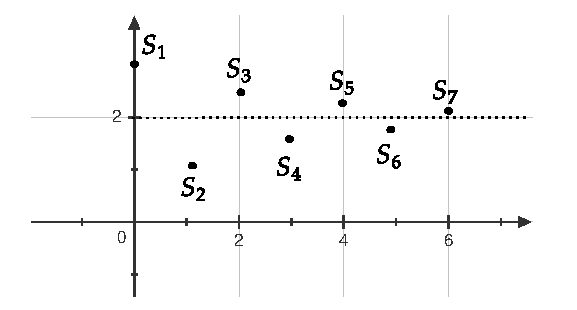
\includegraphics[width=0.8\textwidth]{alternating.pdf}
\end{center}

\begin{Example}{}{}
    Determine whether the following series is convergent or divergent.
    \begin{enumerate}[label=(\roman*)]
        \item $ \displaystyle  \sum\limits_{n=1}^{\infty} \frac{(-1)^{n+1}}{n} $
              (\emph{Alternating Harmonic Series})

              \textbf{Solution.} First, $ \dfrac{1}{n+1}<\dfrac{1}{n} $,
              so $ \set*{\dfrac{1}{n}} $ is decreasing. Also,
              $ \lim\limits_{{n} \to {\infty}} \dfrac{1}{n}=0 $. So,
              the Alternating Harmonic Series converges by AST\@.
        \item $ \displaystyle \sum\limits_{n=2}^{\infty} \frac{(-1)^n}{n\ln(n)} $

              \textbf{Solution.}
              First, $ \dfrac{1}{(n+1)\ln(n+1)}\leqslant \dfrac{1}{n\ln(n)} $,
              so $ \set*{\dfrac{1}{n\ln(n)}} $ is decreasing. Also,
              $ \lim\limits_{{n} \to {\infty}} \dfrac{1}{n\ln(n)}=0 $. So,
              the series converges by AST\@.
    \end{enumerate}
\end{Example}
Q\@: What if we are dealing with alternating series, but it doesn't satisfy
the hypotheses of the AST?! It's our only test!

A\@: If an alternating series fails the AST, it means you forgot to check the Divergence Test!

See the following example.
\begin{Example}{You forgot to check the Divergence Test!}{}
    Is
    $ \displaystyle  \sum\limits_{n=1}^{\infty} \frac{(-1)^n e^{2n}}{e^{2n}+1} $
    convergent or divergent?

    \textbf{Solution.}
    Using the Divergence Test:
    \[ \lim\limits_{{n} \to {\infty}} \frac{(-1)^n e^{2n}}{e^{2n}+1}=
        \lim\limits_{{n} \to {\infty}} \frac{(-1)^n}{1+\sfrac{1}{e^{2n}}} \]
    does not exist. Thus, the series diverges.
\end{Example}

\subsection*{Estimating Sums of Alternating Series}
Suppose we have an alternating series $ \sum\limits_{n=1}^{\infty} (-1)^{n+1}a_n $
that converges by AST\@.

We know from the proof that the odd partial sums approach the actual sum from above,
while the even partial sums approach from below.

This means the actual sum lies between any two consecutive partial sums,
so the error satisfies
\[ \abs*{R_n}=\abs{S-S_n}\leqslant \abs*{S_{n+1}-S_n}=\abs*{\pm a_{n+1}}=
    a_{n+1} \]
which is the next term! So, $ \boxed{\abs*{R_n}\leqslant a_{n+1}} $.

\begin{Example}{}{}
    Find an upper bound on the remainder if we use $ S_{10} $ to approximate
    $ \displaystyle \sum\limits_{n=1}^{\infty} \frac{(-1)^{n+1}}{n} $.

    \textbf{Solution.} $ \abs{R_n}\leqslant a_{n+1} $, so $ \abs{R_{10}}\leqslant a_{11}=\sfrac{1}{11} $.
\end{Example}

\begin{Example}{}{}
    How many terms are needed to approximate
    $ \displaystyle  \sum\limits_{n=1}^{\infty} \frac{(-1)^n}{10^n n!} $
    with an error of at most $ 0.000005 $?

    \textbf{Solution.} The series converges by AST (exercise)
    \[ \abs{R_n}\leqslant a_{n+1}=\frac{1}{10^{n+1}(n+1)!}, \]
    so we want $ a_{n+1}\leqslant 0.000005 $. Guess and check
    (since factorials don't have inverses).
    \begin{itemize}
        \item $ n=3 $: $ \dfrac{1}{10^4(4)!}\approx 0.000004 $ (good!)
        \item $ n=2 $: $ \dfrac{1}{10^3(3)!} \approx 0.0016 $ (bad!)
    \end{itemize}
    So $ n=3 $ works (3 terms).
\end{Example}

Q\@: Is the 121st partial sum of
$ \displaystyle  \sum\limits_{n=1}^{\infty} \frac{(-1)^{n+1}3^n}{(n) 4^n} $
an overestimate or underestimate of the actual sum?

A\@: First term is positive, so the odd partial sums are
above the sum while the even partial sums are below. So
$ S_{121} $ is an \emph{overestimate}!

\begin{Remark}{}{}
    If the first term is negative, then the odd partial sums are underestimates
    while the even partial sums are overestimates.
\end{Remark}
